\chapter{Geofysik}

\section{Introduktion}
I geofysik benytter man fysikkens love og metoder til at undersøge atmosfæren og jordens sammensætning og alder. Geofysik blander praktisk og teoretisk arbejde, hvor teorien man arbejder med primært er specificeret til det, som man vil undersøge. Det er sjældent et teoretisk tungt fag, men der gøres meget brug af teknisk viden og anvendelse af teori til at opbygge modeller af jorden, samt beskrive hvordan den kan undersøges.\\ \\
%
%
Man kan f.eks. via seismologi måle på lydbølger i jorden, og derved detektere jordskælv. Man kan også datere stens alder via radioaktivitet og derefter stykke modeller sammen, der beskriver hvordan Jordens tektoniske plader har bevæget sig og hvornår Jorden har været under istiderne.\\
%
I geofysik arbejder man også med modellering af luft og væsker. Dette kan være alt fra grundvandsstrømning og modellering af forurening i grundvand til modellering af atmosfærens jetstrømme og hvilken effekt klimaændringerne har på dem. \\ \\
%
%
Her på campen vil vi med emnet tage udgangspunkt i praktisk arbejde, med forsøg der gør brug af laboratoriearbejde og feltarbejde. Teorien vi har vil kun være til for at give en forståelse nødvendig for at udføre disse forsøg. \\ \\
%
%
Vi vil tage udgangspunkt i resistivitetsmålinger, dvs. målinger af jordens specifikke elektriske modstand. Disse går kort fortalt ud på at sende strøm ned gennem jorden. Ud fra den specifikke modstand man måler, og hvilke afstande man har mellem måleinstrumenterne i opstillingen, kan man så finde frem til hvilke jordlag, der befinder sig under opstillingen, samt hvor dybt de er nede i jorden.

\section{Teori}

\subsection{Modstand og resistivitet} \label{ting}
Elektrisk modstand, eller resistans, beskriver, hvordan strøm, der løber gennem et materiale, oplever en modstand mod sin bevægelse. Her omdannes elektrisk energi til varmeenergi grundet urenheder i materialet, som begrænser strømmens gennemløbsareal. Fænomenet kan sammenlignes med vandstrøminger, se figur~\ref{fig:geo_hydraulican}.
\begin{figure}[h]
    \centering
    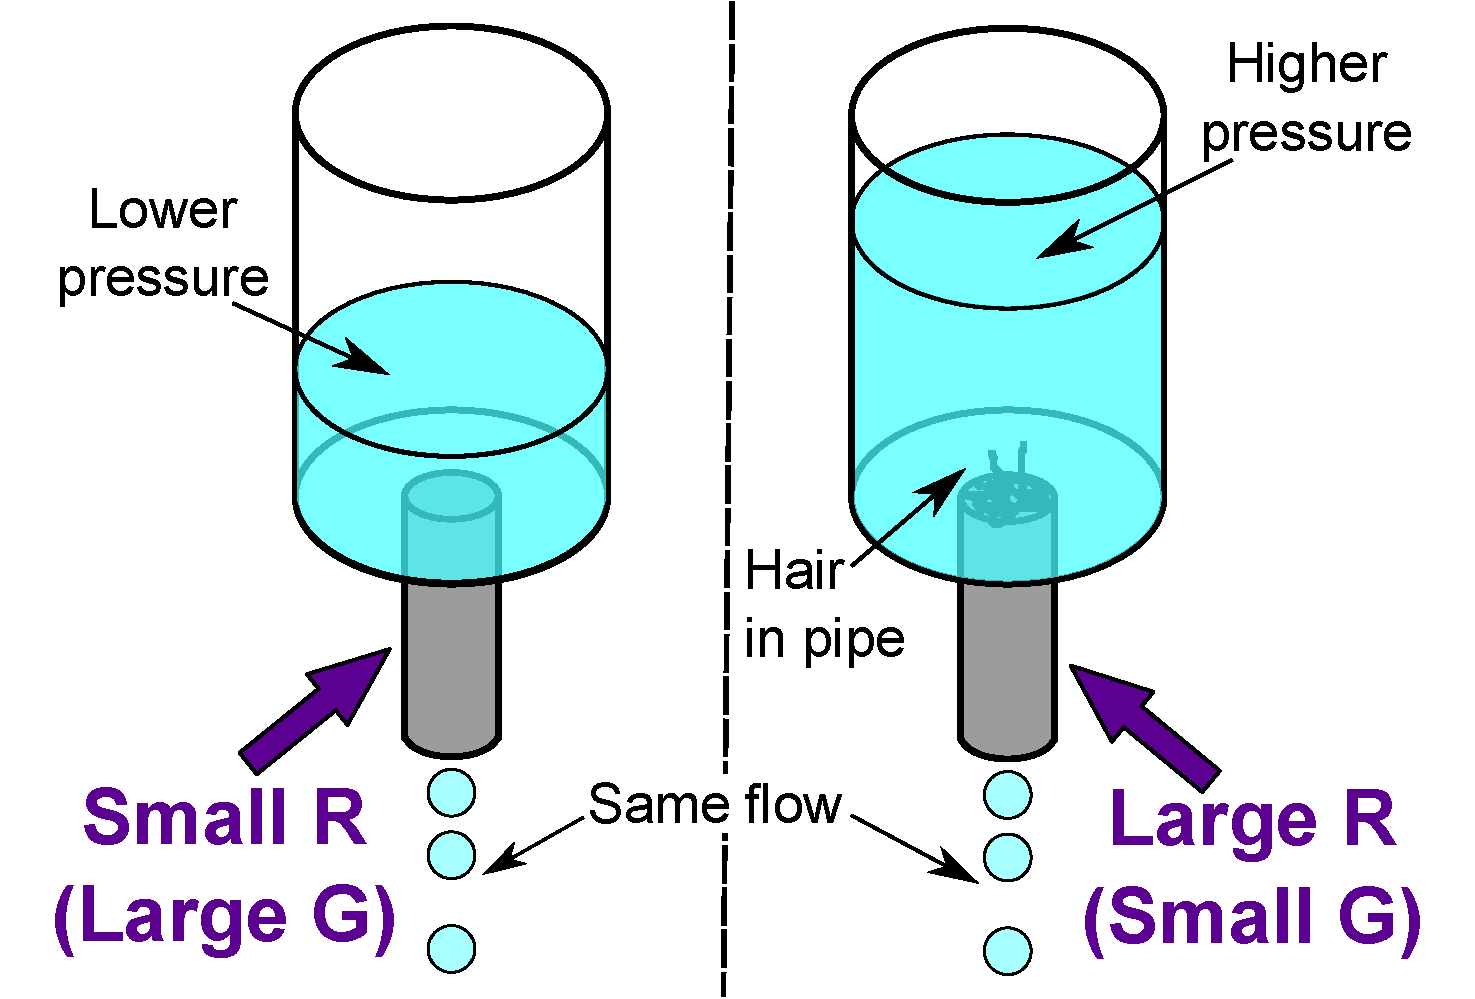
\includegraphics[width = 0.7\textwidth]{Geo/Figurer/ResistanceHydraulicAnalogy.pdf}
    \caption{Analogi til resistans: På figuren er der to opstillinger. På den venstre er der vand i en beholder, med et rør (ledning) hvorigennem vandet løber ud af beholderen med en vis hastighed, altså en vis strøm. Hvis dette rør pludselig begynder at blive blokeret (højreside, f.eks. af hår), så løber vandet langsommere igennem (lavere strømning), da det effektive ledningsareal nu er lavere. For at få samme strømning som før, så skal der kompenseres ved at øge trykket i røret, og derved have mere vand i beholderen. Dette svarer til at øge spændingen over ledningen, hvis det var en elektrisk strøm. Kilde: \cite{ElectricalResistanceConductance}.
    }
    \label{fig:geo_hydraulican}
\end{figure}

Elektrisk resistans gennem et stykke ledning beskrives ud fra Ohm's lov:
\begin{align}\label{eq:geo_ohm}
    R = \frac{V}{I}.
\end{align}
Her er $I$ strømmen gennem ledningsstykket, $R$ er resistansen, og $V$ er spændingsforskellen mellem starten og slutningen af ledningen (også blot kaldet spændingen over ledningsstykket). Resistansen afhænger af materialet, som ledningen er lavet af, hvilket er grunden til, at vi gerne vil benytte det til vores målinger. Men ligesom med vandanalogien i figur~\ref{fig:geo_hydraulican}, så afhænger den også af tykkelsen af ledningen (da den afhænger af strømningen gennem ledningen), samt længden af ledningen (da den afhænger af spændingsfaldet over ledningsstykket). Dette gør resistansen upraktisk at måle, når vi ikke arbejder med ledningsstykker, men i stedet arbejder med jordlag i felten. \\ \\
%
%
Derfor indføres nu et begreb ved navn resistivitet, eller specifik elektrisk modstand. Specifik elektrisk modstand er, ligesom f.eks. massefylde, også kaldet densitet, en materialeegenskab. Den betegnes $\rho$ og kan på sin simpleste form beskrives for et pænt kasseformet materiale ud fra ligningen
\begin{align}
    \rho = R \frac{A}{l}.
\end{align}
Her er $R$ den elektriske resistans (ligesom før), $l$ er længden af materialet, og $A$ er tværsnitsarealet gennem materialet (svarende til tykkelsen af ledningen). Se figur~\ref{fig:geo_resistans} for en illustration af størrelserne.
\begin{figure}[h]
    \centering
    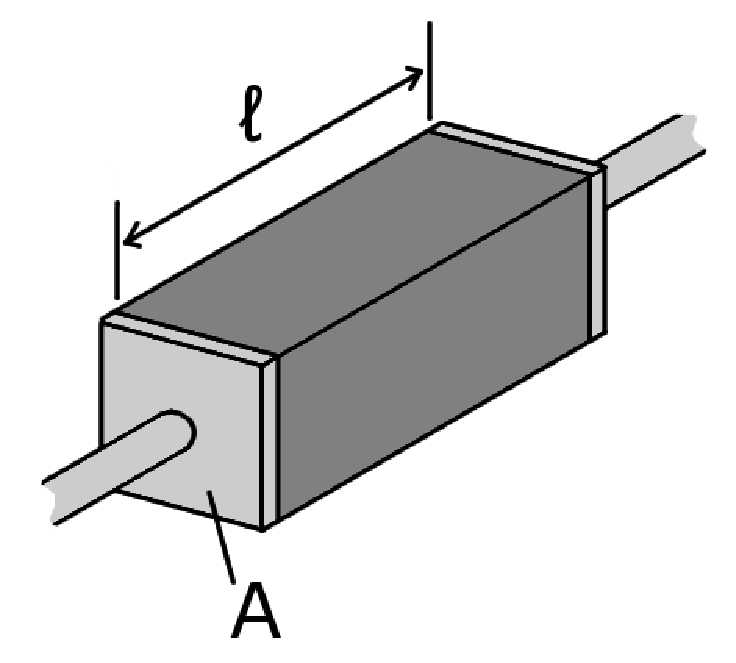
\includegraphics[width = 0.5\textwidth]{Geo/Figurer/resistivity_geometry.pdf}
    \caption{Et stykke resistivt materiale (mørkegrå) med elektrisk kontakt (lysegrå) i begge ender, hvor der udelukkende måles resistivitet for materialet. Indlagt er tværsnitsareal A, samt materialelængde l.
    Kilde: \cite{ElectricalResistanceConductance}.}
    \label{fig:geo_resistans}
\end{figure}
Det gode ved resistiviteten er, at den for et ensartet, jævnt materiale (også kaldet et homogent materiale), altid har den samme værdi, ligegyldigt hvilken form, som materialet har. Hvis vi kan finde en solid og god måde at bestemme resistiviten af de materialer, som måler på, så vil vi netop få de samme målinger uafhængigt af, hvor meget materiale vi kommer igennem og hvor dybt vores strøm kommer ned (medmindre vi nu kommer langt nok ned til at ramme et nyt jordlag, der har en anden resistivitet).
%
\subsection{Måling af resitivitet}
Forestil dig, at man har et meget dybt og bredt jordlag (vi antager at det er uendeligt dybt og bredt), og at vi lige oven på jordlaget har placeret en strømkilde (elektrode), f.eks. enden af en ledning.
Hvis dette jordlag alle steder er ensartet (samme densitet og opbygning. Specielt samme elektriske egenskaber), så kaldes det homogent. \\
%
\begin{figure}
	\centering
	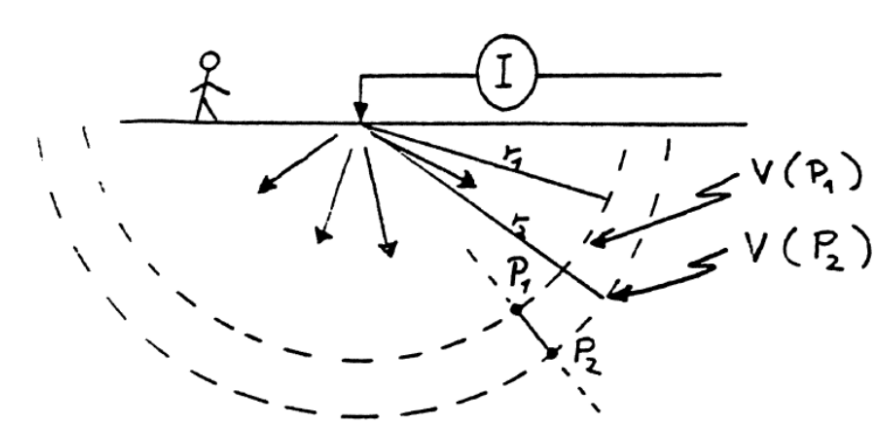
\includegraphics[width=\textwidth]{Geo/Figurer/halvcirkel.png}
	\caption{Figuren viser en jordoverflade, med et homogent jordlag nedenunder, og en enkelt elektrode koblet til. Pilene illustrerer strømmens retning. De stiplede linjer illustrerer punkter, der har samme afstand til elektroden, og derved samme elektriske potential (spænding).}
	\label{fig:geo_halvcirkel}
\end{figure}
Strømkilden er sådan set blot en tilførsel af ladning, så når den forbindes til jorden, vil ladningen sprede sig ud gennem det neutralt ladede jordlag, og der vil løbe en strøm ud i jorden. Hvis jordlaget er homogent, så vil der med sikkerhed ikke være nogen betydelig, foretrukken vej for ladningen at bevæge sig, og strømmen vil derfor løbe ensartet ud i alle retninger, se figur \ref{fig:geo_halvcirkel}. Dette betyder, at strømtætheden i jorden vil falde som funktion af radius (på en kugle), som vi kommer væk fra strømkilden. Da der ikke kan løbe en strøm ovenover jordoverfladen (hvor der kun er luft, som ikke kan lede strømmen), må strømtætheden være dobbelt så stor, som hvis strømmen kunne løbe i alle retninger. Strømtætheden $J$ udtrykkes således ud fra overfladearealet på en halvkugle, $A_{hk}$:
\begin{align}
    A_{hk} &= \frac{1}{2} A_k \\
    A_k &= 4\pi r^2 \\
    A_{hk} &= 2\pi r^2 \\
    J(r) &= \frac{I}{A_{hk}} = \frac{I}{2\pi r^2}.\label{eq:geo_Jr}
\end{align}
Her er $A_k$ overfladearealet af en kugle, $I$ er den tilførte strømstyrke, og $r$ er radius af kuglen. \\

%
En mere generel måde at definere resistiviteten $\rho $ på (hvilket giver det samme, som i vores mere ideelle tilfælde fra tidligere) er ud fra en ligning, som beskriver sammenhængen mellem strømtætheden $J$ og det elektriske felt $E$ produceret af vores strømkilde i jorden:
\begin{align}\label{eq:geo_EJ}
    E &= \rho J.
\end{align}
Vores resistivitet er fast for materialet, så længe materialet er homogent (ensartet). I dette tilfælde har vi at $J$ (og derved $E$) udelukkende afhænger af radius, og der er derfor sfærisk (kugle) symmetri. Hvis strømstyrken $I$ er konstant, så vil følgende sammenhæng mellem det elektriske potential $V$ (spænding) og det elektriske felt $E$ gælde (ud fra en definition af det elektriske felt):
\begin{align}
    E = - \pdv{V}{r}.
\end{align}
Ved hjælp af ligningerne \eqref{eq:geo_Jr} og~\eqref{eq:geo_EJ} får vi så
\begin{align}
    \rho J(r) &= - \pdv{V}{r} \\
    \rho \frac{I}{2\pi r^2} &= - \pdv{V}{r}.
\end{align}
For at få et udtryk for det elektriske potential $V(r)$ skal vi således integrere begge sider af ligningen, altså mht. r. Til at gøre dette vælger vi at finde potentialforskellen mellem to punkter i afstandene hhv. $r_1$ og $r_2$:
\begin{align}
    V(r_2) - V(r_1) &= \int_{r_1}^{r_2} \frac{-\rho I}{2\pi} \frac{1}{r^2} dr \\ \nonumber
                    &= -\frac{\rho I}{2\pi} \int_{r_1}^{r_2} \frac{1}{r^2} dr \\ \nonumber
                    &= -\frac{\rho I}{2\pi} \left[-\frac{1}{r}\right]_{r_1} ^{r_2} \\ \nonumber
                    &= \frac{\rho I}{2\pi} \left(\frac{1}{r_2} - \frac{1}{r_1}\right).
\end{align}
Nu kan vi så fastsætte, hvad vi ønsker de to afstande til at være, afhængigt af, hvor vi starter henne. Vi vil gerne have, at potentialet skal være positivt, men 0 når vi er uendeligt langt væk, da dette betyder at potentialet er maksimalt tæt ved elektroden. Så vi sætter $r_2 = r$, og $r_1 = \infty$ og får
\begin{align}\label{lign:geo_potentiale}
    V(r) &= \frac{\rho I}{2\pi r}.
\end{align}
Dette er gyldigt, fordi vi i vores tidligere udregninger blot havde regnet ud fra to vilkårlige punkter $r_1$ og $r_2$, hvor vi nu har valgt at specificere $r_1$ til at være der, hvor $V = 0$, dvs. $r_1 = \infty$. \\
%
Nu har vi altså fundet et udtryk for det elektriske potential i et homogent jordlag for en enkelt strømkilde afhængigt af resistivitet $\rho$ af materialet, strømstyrke $I$ af kilden, samt afstand $r$ fra kilden. \\ \\
%
%
Hvad så hvis vi har to elektroder (strømkilder) i jordoverfladen, med en afstand $L$ i mellem sig, og som har ens men modsatrettet strøm, henholdsvis $I$ og $-I$ løbende? (Dette svarer til et kredsløb, hvor en anode og katode sættes i jorden, nærmere sagt en positivt og negativt ladet elektrode forbundet i kredsløb gennem jorden). \\ \\
%
%
Lad os sige, at vi ønsker at finde det elektriske potential ved et vilkårligt punkt P i jorden. \\
%
I dette tilfælde kan potentialet fra hver enkelt elektrode beskrives separat vha. ligning~\eqref{lign:geo_potentiale}. For at finde det samlede potentiale skal man derved blot lægge de to elektroders påvirkning sammen (kaldet superpositionsprincippet). Hvis den første elektrode ($+I$) har en afstand $r_1$ til punktet, man ønsker at finde potentialet i, og den anden elektrode ($-I$) har en afstand $r_2$ til punktet, så får man det totale potential til at være
\begin{align}\label{eq:geo_Vdipol}
    V(P) &= \frac{\rho I}{2\pi r_1} + \frac{\rho \cdot (-I)}{2\pi r_2} \\
        &= \frac{\rho I}{2\pi r_1} - \frac{\rho I}{2\pi r_2}.\label{eq:geo_Jr}
\end{align}
Det kan her ses, at selvom vi har valgt et meget specifikt punkt, så afhænger resultatet kun af afstanden til de to elektroder. Det vil sige, at hvis vi kan finde et andet punkt, der har samme afstand til de to elektroder, så vil vi få samme potential. Dette skal vi benytte når, vi skal lave såkaldte 4-polsopstillinger.
%
%
\subsection{4-polsopstilling}\label{ssec:4-pols opstilling}
Forestil dig en opstilling, hvor vi nu har 4 elektroder i forbindelse med jordoverfladen. To af dem er forbundet i et kredsløb, hvor der løber en strøm, $I$, fra den ene til den anden (situationen fra før). De er placeret i punkterne hhv. $A$ (strømstyrke $+I$) og $B$ (strømstyrke $-I$) på overfladen. Mellem dem er der yderligere to elektroder, der ikke er koblet til en ekstern strømkilde, men bruges til at måle et spændingsfald $\Delta V$. Disse elektroder ligger i punkterne $C$ og $D$ på overfladen ($C$ er tættest på $A$). En illustration af dette kan ses på figur~\ref{fig:Wenneropstilling}, der viser et eksempel på en sådan opstilling (Wenneropstillingen). Ud fra ligning~\eqref{eq:geo_Vdipol} kan vi så opskrive det elektriske potential ved hhv. $C$ og $D$:
%
\begin{align}
    V(C) &= \frac{\rho I}{2\pi r_{AC}} - \frac{\rho I}{2\pi r_{BC}}, \\
    V(D) &= \frac{\rho I}{2\pi r_{AD}} - \frac{\rho I}{2\pi r_{BD}}, \\
\end{align}
%
samt potentialforskellen mellem dem:
%
\begin{align}
    \Delta V = V(C) - V(D) = \frac{\rho I}{2\pi}\left( \frac{1}{r_{AC}} - \frac{1}{r_{AD}} - \frac{1}{r_{BC}} + \frac{1}{r_{BD}} \right).
\end{align}
%
Vi kan måle strømstyrken, $I$, gennem elektroderne A og B, måle spændingsfaldet $\Delta V$ over C og D, samt måle afstandene mellem elektroderne, så kan vi nu finde et udtryk for resistiviteten af jordlaget (under antagelsen om, at det er homogent, dybt og bredt):
\begin{align}
    \rho &= \frac{2\pi}{1/r_{AC} - 1/r_{AD} - 1/r_{BC} + 1/r_{BD}} \frac{\Delta V}{I} = K \frac{\Delta V}{I},\label{eq:geo_rho}
\end{align}
hvor proportionalitetskonstanten $K$ kun afhænger af den relative placering af elektroderne og kaldes den geometriske faktor for elektrodeopstillingen. Hvis man har et homogent og stort lag, så vil ændringen i $K$, når man flytter rundt på elektrodeopstillingen, kompensere for ændringen i $\Delta V/I$ og sikre, at man får resistivitet hver gang. Ud fra resistiviteten kan man så bestemme, hvilket materiale som laget består af. Dette kan man, da jordlagets resistivitet afhænger af lagets mineralsammensætning og vandindhold (porevand), samt af indholdet af opløste salte (ioner) i porevandet. Derved kan resistiviteten bruges til at indikere, hvilken type jordlag, som vi måler på.
%
\begin{figure}
    \centering
    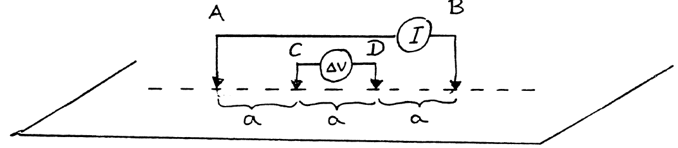
\includegraphics[width=0.8\textwidth]{Geo/Figurer/Wenner-opstilling.png}
    \caption{Her ses Wenneropstillingen, der tager udgangspunkt i, at afstanden mellem hver elektrode og dens nabo-elektroder er ens, $a$, for alle elektroderne.}
    \label{fig:Wenneropstilling}
\end{figure}
%
\subsubsection{Tilsyneladende resistivitet}
Hvad gør man, hvis undergrunden i virkeligheden ikke er homogen? For eksempel, hvis der er mere end et jordlag, som hver især kan ses som homogene, men har forskellige resistiviteter imellem sig. Her giver det stadig mening, at regne den størrelse ligning~\eqref{eq:geo_rho} giver os, hvilket er den samlede resistivitet med forskellige bidrag fra lagene. I stedet for at kalde den resistiviteten, vælger man så, at kalde den for den tilsyneladende resistivitet $\rho_a$, som så er det, som resistiviteten ville være, hvis undergrunden var homogen og bestod af ét lag:
\begin{align}
    \rho _a &= K \frac{\Delta V}{I}.
\end{align}
Bemærk her, at denne ikke er konstant, men er afhængig af, hvordan vores elektrodeopsætning er, da antagelsen om at strømmen løber lige meget i alle retninger ikke er fornuftig længere. Denne variation kan også benyttes, da den kan være med til at fortælle os hvilke jordlag, der ligger i hvilke dybder. For at give en ide om dét, så tager vi her et par tænkte eksempler:\\\\
%
%
Vi har to separate homogene jordlag (f.eks. ler og sand), et ovenpå det andet. Hvis afstanden mellem elektroderne er lille i forhold til tykkelsen af det øverste jordlag, så vil antagelsen om en sfærisk jævn strømning gennem jordlaget være god, da vi nærmer os den antagelse vi lavede i starten om et uendeligt stort homogent lag. Det betyder, at den tilsyneladende resistivitet, vi måler, $\rho_a$, vil være tæt på det samme som den faktiske resistivitet, $\rho$, for det øverste jordlag. Se figur~\ref{fig:geo_ex1} for illustration af dette. \\
%
Hvis vi nu i stedet betragter tilfældet, hvor det øverste lag er tyndt i forhold til afstanden mellem elektroderne, og det nederste lag er tykt (det er lettest at sige uendeligt tykt), så vil strømmen kun have en meget kort vej igennem det øverste lag. Så medmindre resistiviteten i det øverste lag er meget mindre (eller meget større) i forhold til resistiviteten i det nederste lag, så vil det øverste lags indflydelse på den tilsyneladende resistivitet være lille. Men dette må betyde, at siden det nederste lag er homogent, så er den tilsyneladende resistivitet, vi måler, ret tæt på den faktiske resistivitet af det nederste lag. Se figur~\ref{fig:geo_ex2} for illustration af dette tilfælde.\\ \\
%
%
\begin{figure} [h!]
\centering
\begin{minipage}{.95\textwidth}
    \centering
    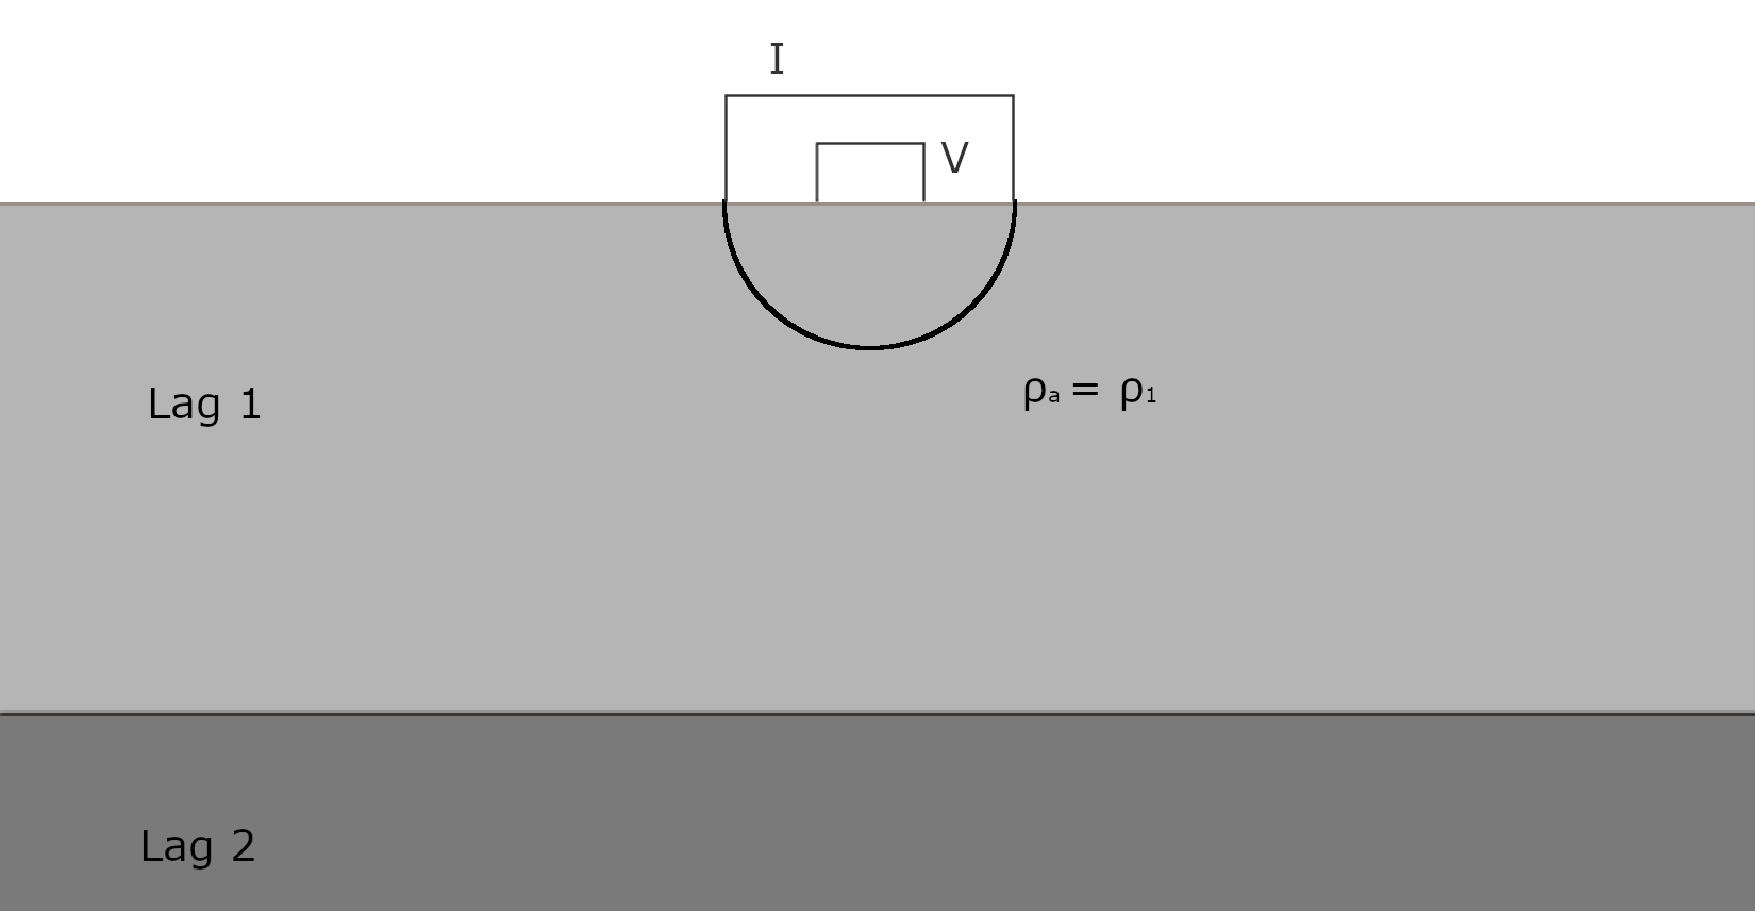
\includegraphics[width = .75\linewidth]{Geo/Figurer/geo_ex1.pdf}
    \captionof{figure}{På denne figur ses et meget tykt førstelag, hvor 4-polsopstillingens diameter er meget lille i forhold til dette. Ved dette vil den tilsyneladende resistivitet, vi måler, således være lig med, eller meget tæt på, den faktiske resistivitet af det øverste jordlag, da den praktisk talt ikke vil være påvirket af resistiviteten af det dybere lag.}
    \label{fig:geo_ex1}
\end{minipage}
\begin{minipage}{.95\textwidth}
    \centering
    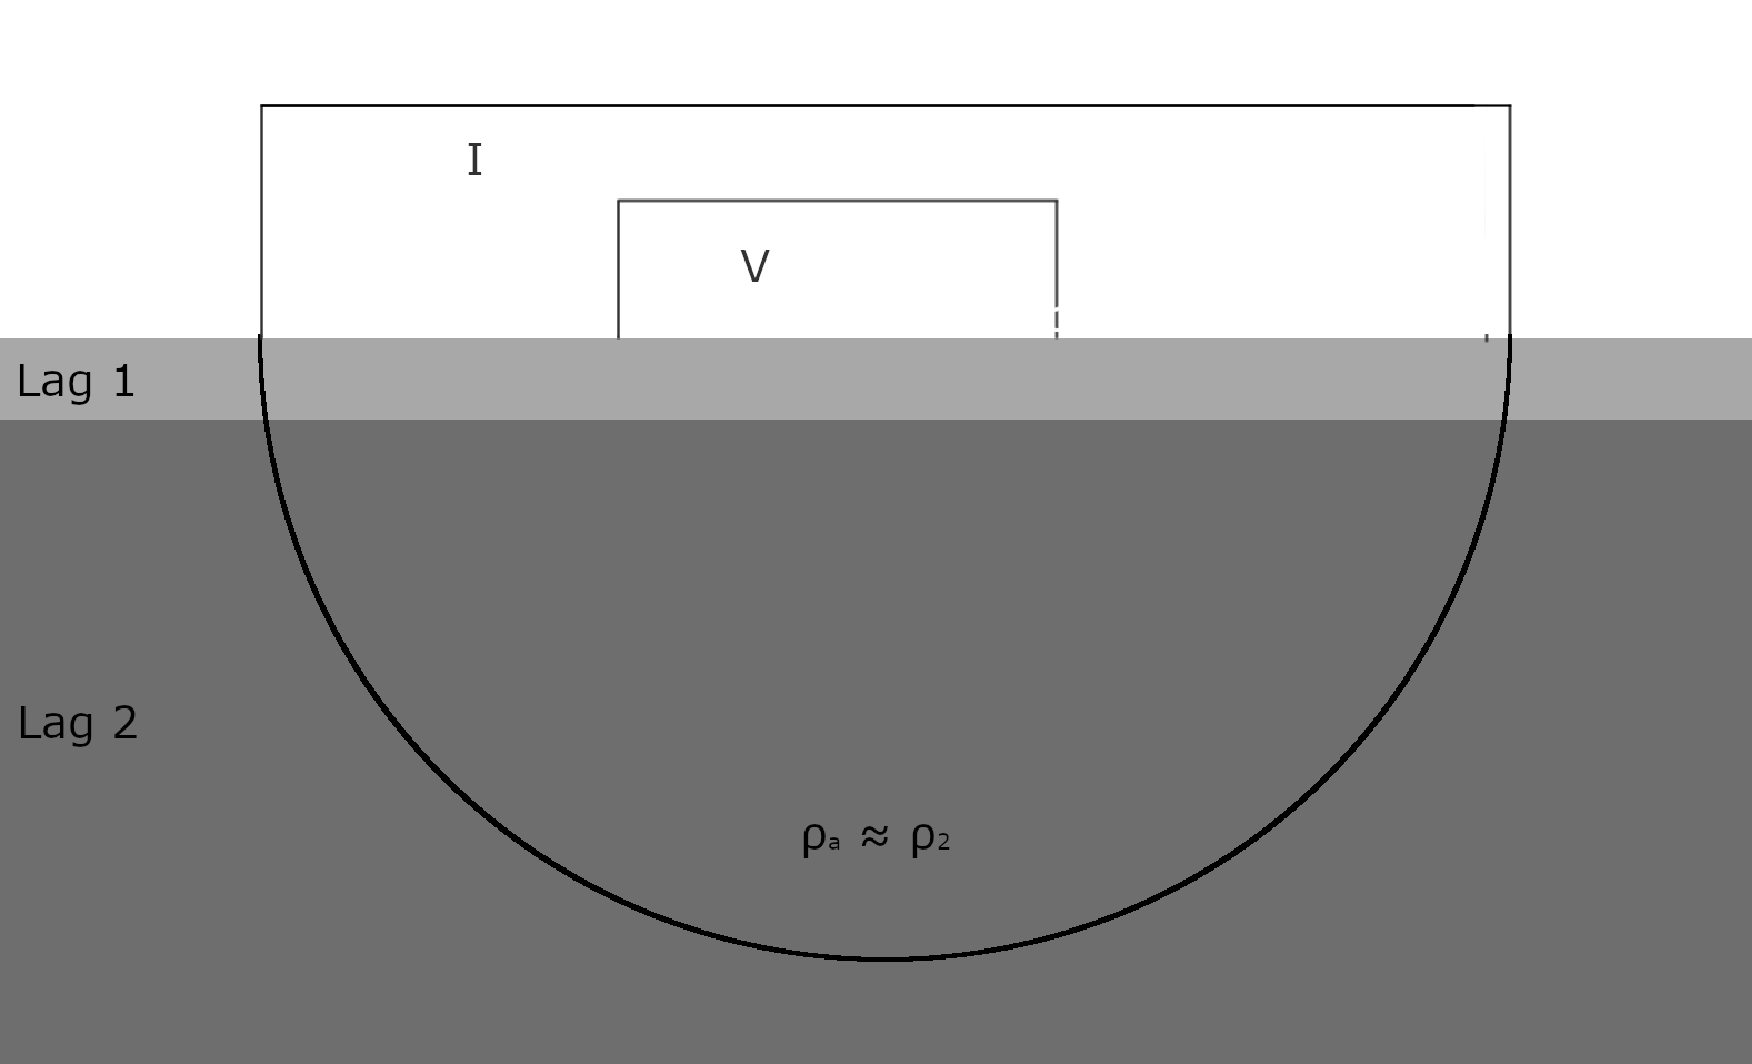
\includegraphics[width = .75\linewidth]{Geo/Figurer/geo_ex2.pdf}
    \captionof{figure}{På denne figur er det øverste lag meget tyndt i forhold til både afstanden mellem elektroderne og tykkelsen af det nederste lag. Dette betyder, at medmindre resistivitetsforskellen mellem de to lag er meget stor (meget høj resitivitet af lag 1 mod meget lav resistivitet af lag 2, eller omvendt), så vil den tilsyneladende resistivitet være approksimativt lig resistiviteten i det 2. lag.}
    \label{fig:geo_ex2}
\end{minipage}
\end{figure}
\\
På den måde kan den tilsyneladende resistivitet ses som værende et vægtet gennemsnit af resistiviteten af de lag, som vi sender strøm igennem. Vægtningen afhænger således af hvilket volumen, vores opstilling udspænder. Den afhænger også af forskellen mellem resistiviteten i lagene.
\\
\begin{figure}[h!]
    \centering
    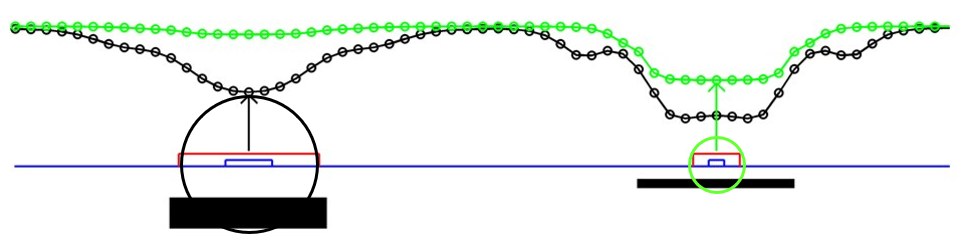
\includegraphics[width=0.8\textwidth]{Geo/Figurer/Big-small_resistivity_curve.png}
    \caption{På denne figur ses to 4-polsopstillinger, en med stor elektrodeafstand og en med lille. Opstillingerne står på et homogent lag, hvori der er to objekter, et dybt og tykt og et tæt på overfladen og smallere. Begge objekter har samme resistivitet. Den grønne kurve viser data fra den lille opstillings tilsyneladende resistivitetsmålinger, og den sorte viser den store opstillings målinger. Den lille opstilling giver kun et udsving ved det overfladenære objekt, da den ikke når ned til det dybe objekt. Den store opstilling rammer derimod begge objekter, men giver en mindre præcis lokation, specielt på det overfladenære objekt.}
    \label{fig:Big-small resistivity curve}
\end{figure}
\\ \\ \\ \\ \\ \\ \\ \\ \\
\subsubsection{Wenneropstillingen}
 Man kan lave mange forskellige 4-polsopstillinger, men nogle af dem er standardiserede, så man nemt kan finde den geometriske faktor.
 En af de mere simple, og den der i dette emne bliver arbejdet med, er Wenneropstillingen (figur~\ref{fig:Wenneropstilling}), som er en simpel og fleksibel opstilling. Wenneropstillingen tager udgangspunkt i, at man holder afstanden mellem elektroderne konstant, således at afstanden mellem to naboelektroder altid er lig en konstant afstand $a$. Således bliver den samlede længde af 4-polsopstillingen $3a$. \\
 %
 Wenneropstillingens største svaghed er, at når man kommer op på store afstande, så bliver man nødt til at have meget lange kabler, og modellen er derved ikke lige så skalerbar arbejdsmæssigt. \\
 %
 For at kunne bruge Wenneropstillingen, skal man kende dens geometriske faktor. Den generelle formel for den geometriske faktor blev fundet i afsnittet om 4-polsopstillinger i ligning~\eqref{eq:geo_rho}, til \\
 \begin{align}
     K&=\frac{2\pi}{1/r_{AC} - 1/r_{AD} - 1/r_{BC} + 1/r_{BD}}. 
 \end{align}
Herfra kan man man så bytte $r$ ud med $a$, og så får man
\begin{align}
     K&=\frac{2\pi}{1/a - 1/2a - 1/2a + 1/a} = 2\pi a.
 \end{align}
Vi får derfor en geometrisk faktor, som kun afhænger af $a$. \\ \\
%
%
I Wenneropstillingen sender man en strøm, $I$, igennem jorden fra A til B, hvorefter man måler spændingsfaldet, $\Delta V$, fra C til D. Du kan læse om dette i afsnittet omkring 4-polsopstillingen, afsnit~\ref{ssec:4-pols opstilling}.
%

\subsubsection{Profilering og Sondering} \label{Profilering og Sondering}
Der er to forskellige måder at foretage målinger med Wenneropstillingen (og andre 4-polsopstillinger), som bruges til forskellige formål. De tager udgangspunkt i hvad der kan varieres, når der tages flere målinger; hhv. placeringen af alle elektroderne (hvor afstanden mellem dem holdes fast), og afstanden mellem elektroderne (hvor centrum af opstillingen holdes fast). \\ \\
%
%
Den første kaldes geoelektrisk profilering. Ved denne holder man afstanden mellem elektroderne fast, hvilket betyder at man holder en konstant måledybde. Samtidig flytter man opstillingen rundt, hvorved man så kan måle og optegne et kort eller en profil for undergrunden i en bestemt dybde. For at få et visuelt billede, kan figur~\ref{fig:Wenneropstilling} bruges. Forestil dig her, at man, efter at have taget en måling, flyttede hele opstillingen langs den stiplede linje. På den måde ville man kunne kortlægge jordlagene på en vis dybde, langs den stiplede linje.\\ \\
%
%
Den anden metode kaldes geoelektrisk sondering. Her holdes centrum af opstillingen, og derved placeringen af målingen, fast. Til gengæld ændres afstanden mellem elektroderne, og derved dybden af målingen. Man skaber således med mange målinger en model for, hvordan undergrunden ser ud lodret ned under opstillingen. For at få et visuelt billede af sondering, kan figur~\ref{fig:geo_ex1} og figur~\ref{fig:geo_ex2} bruges, hvis der ses bort fra at jordlagene er forskellige i de to figurer. \\
De to metoder har som nævnt forskellige formål. Et eksempel på det kan være, hvis man skal kortlægge et vandførende sandlag i undergrunden. Da kan det være brugbart, at starte med en sondering, et sted hvor man ved at laget befinder sig (eller gætter på at det gør). På den måde kan man bestemme dybden af laget. Dernæst kan man profilere med den kendte dybde, og således skabe sig et kort over hvor langt laget strækker sig ud.


\subsection{Tre og flere-lags modeller}
I de tidligere afsnit har vi arbejdet med to lag. I mange situationer vil man arbejde med tre eller flere lag, specielt når man har med sondering at gøre. \\
Hvis man arbejder med flere lag, bruger man de samme teknikker, som til to lag. De bliver dog mere komplicerede. Dette er især tydeligt, hvis man gerne vil finde den specifikke resistivitet, i stedet for den målte tilsyneladende resistivitet. Grunden til at det kan være svært er, at de forskellige lag har indflydelse på lagene omkring dem.\\
%
Den tilsyneladende resistivitet blev tidligere beskrevet som et vægtet gennemsnit af volumen og forskellen i resistiviteten for lagene. Dette kan ses på figur~\ref{fig:Tre-lagsmodel_tilres}. \\ \\
%
%
\begin{figure}
    \centering
    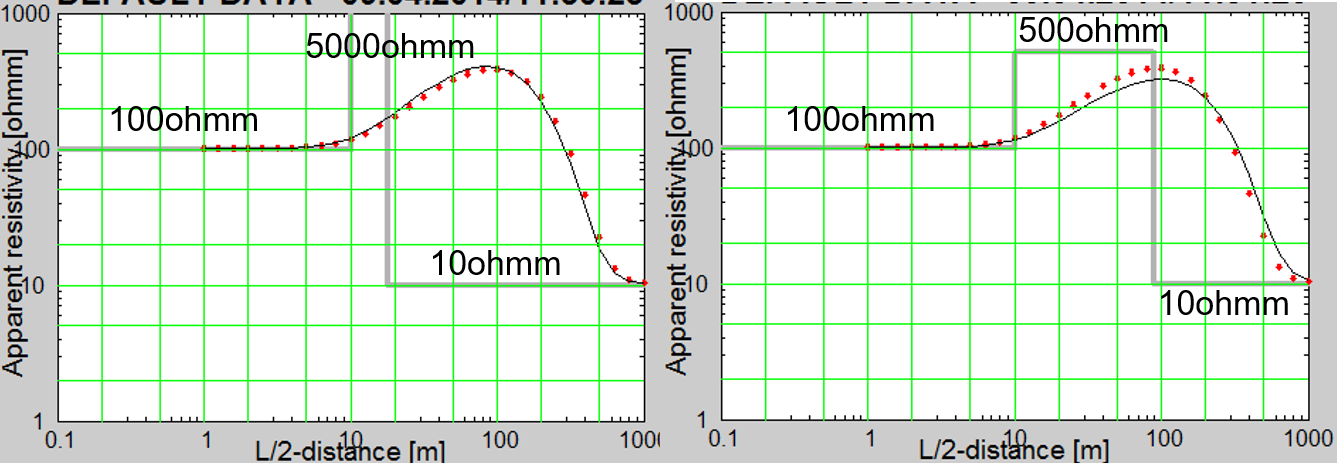
\includegraphics[width=0.8\textwidth]{Geo/Figurer/tilsynelsadet_resistivitet.png}
    \caption{På denne figur ses to tre-lagsmodeller, hvor kun det midterste lag er forskelligt, og man har dybden på $x$-aksen, samt resistiviteten op ad y-aksen. Derudover ses det, at hver trelagsmodel har en tilsyneladende resistivitetskurve, som er næsten ens. Grunden til at den tilsyneladende resistivitet er den samme for begge modeller, er at vægtningen for det midterste lag er ens. Vægtningen afhænger derfor både af resistiviteten og tykkelsen af laget.}
    \label{fig:Tre-lagsmodel_tilres}
\end{figure}
En af udfordringerne, når man arbejder med flere lag, er vægtingen, da man kan have svært ved at finde ud af, om det er tykkelsen eller resistiviteten, som man skal ændre på, for at den tilsyneladende resistivitet passer på ens model. Her kan geologisk forhåndsviden dog hjælpe, da det kan sætte begrænsninger på hvilke modeller, der kan benyttes. \\
%
Et andet potentielt problem kan være, at et lag ikke viser sig i modellen ud fra ens målte resistiviteter. Dette skyldes at vægtningen af dette lag er for lille i forhold til de andres lag. Enten kan laget være for tyndt eller have en for lille forskel i resistivitet i forhold til de omgivende lag.\\
Det kan være svært at finde ud af disse faldgrupper, medmindre at man går ud og borer eller laver nogle mere komplicerede modelleringer. Derfor arbejder man mest på computer, når man arbejder med flere lag. Da de modeller, man har behov for, både er for regnetunge til at kunne udføres i hånden, og fordi fejl i første lag kan fører til større fejl i lagene nedenunder, da de er afhængige af hinanden. Lokal geologisk viden kan desuden inddrages, til at sætte startbetingelser eller begrænsninger på modelleringsprocessen, for derved at få mere præcise modeller.
